
We examine numerically the boundaries \eqref{eq:strong-classification-boundary} under several error tail assumptions for independence errors in this section.
Numerical experiments for dependent errors will be deferred until we characterize the \ac{URS} conditions in Chapter \ref{chap:URS}.

To demonstrate the phase transition phenomenon under different error tail densities, we simulate from the additive error model \eqref{eq:model-additive} with
\begin{itemize}
    \item Gaussian errors, where the density is given by
    $f(x) = \frac{1}{\sqrt{2\pi}}\exp{\left\{-x^2/2\right\}}$.
    \item Laplace errors, where the density is given by $f(x) = \frac{1}{2}\exp{\left\{-\left|x\right|\right\}}$.
    \item Generalized Gaussian $\nu=1/2$, with density
    $f(x) = \frac{1}{2}\exp{\big\{-2\left|x\right|^{1/2}\big\}}$.
\end{itemize}
The sparsity and signal size of the sparse mean vector are parametrized as in equations \eqref{eq:sparsity-parametrized} and \eqref{eq:signal-size-parametrized}, respectively.
The support set $S$ is estimated with 
$\widetilde{S} = \left\{i:x(i)>\sqrt{2\log{p}}\right\}$ 
under the Gaussian errors, 
$\widetilde{S} = \left\{i:x(i)>\log{p} + (\log{\log{p}})/2\right\}$ 
under the Laplace errors, and with
$\widetilde{S} = \{i:x(i)> \frac{1}{4}\left(W\left(-c/(ep\log{p})\right) + 1\right)^2\}$
under the generalized Gaussian ($\nu = 1/2$) errors. Here $W$ is the Lambert W function, i.e., $W=f^{-1}$ where $f(x)=x\exp{(x)}$.
The choices of thresholds correspond to Bonferroni's procedures with FWER decreasing at a rate of $1/\sqrt{\log{p}}$, therefore satisfying the assumptions in Theorem \ref{thm:sufficient}.
Experiments were repeated 1000 times under each sparsity-and-signal-size combination.

The results of the numerical experiments are shown in Figure \ref{fig:phase-simulated}.
The numerical results illustrate that the predicted boundaries are not only accurate in high-dimensions ($p=10000$, right panels of Figure \ref{fig:phase-simulated}), but also practically meaningful even at moderate dimensions ($p=100$, left panels of Figure \ref{fig:phase-simulated}).

\begin{figure}
      \centering
      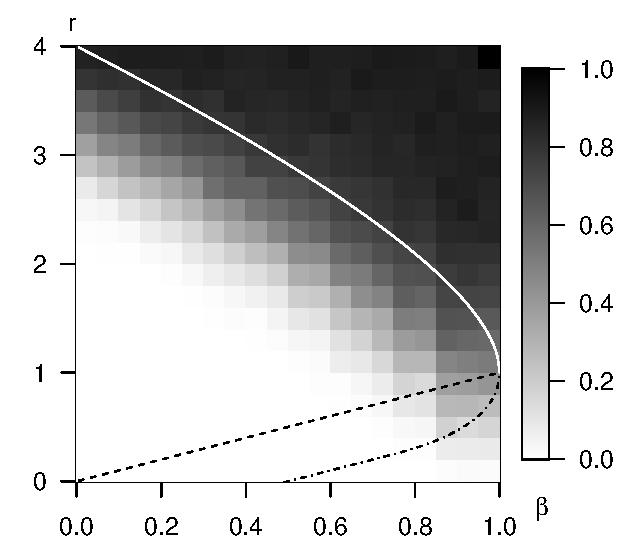
\includegraphics[width=0.4\textwidth]{./figures/simulated_boundaries/simulated_phase_diagram_p100.eps}
      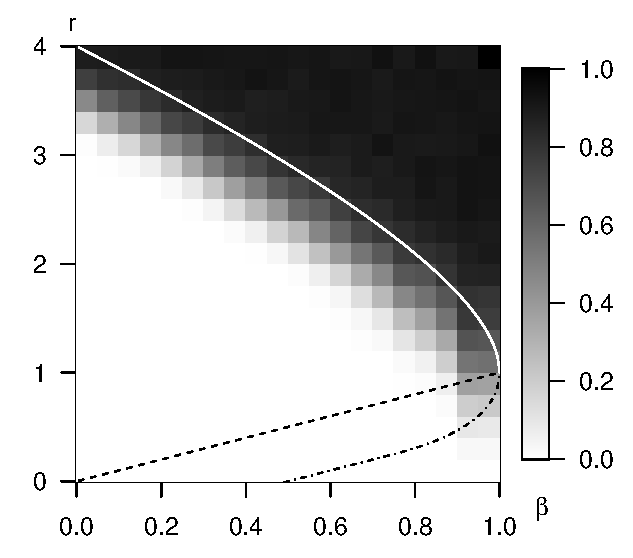
\includegraphics[width=0.4\textwidth]{./figures/simulated_boundaries/simulated_phase_diagram_p10000.eps}
      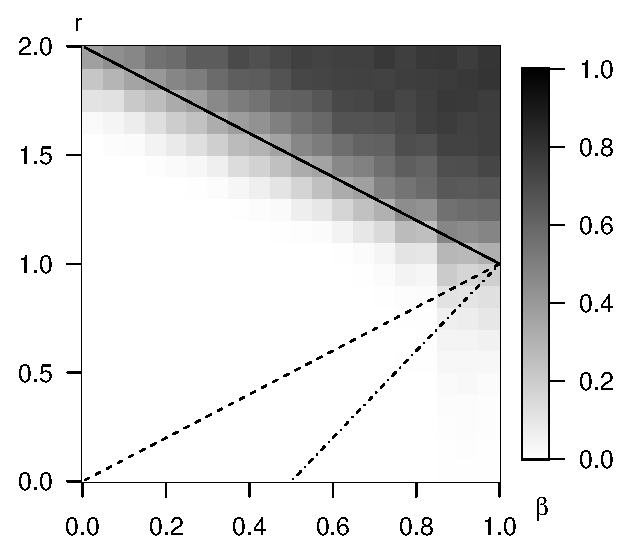
\includegraphics[width=0.4\textwidth]{./figures/simulated_boundaries/simulated_phase_diagram_Laplace_p100_4.eps}
      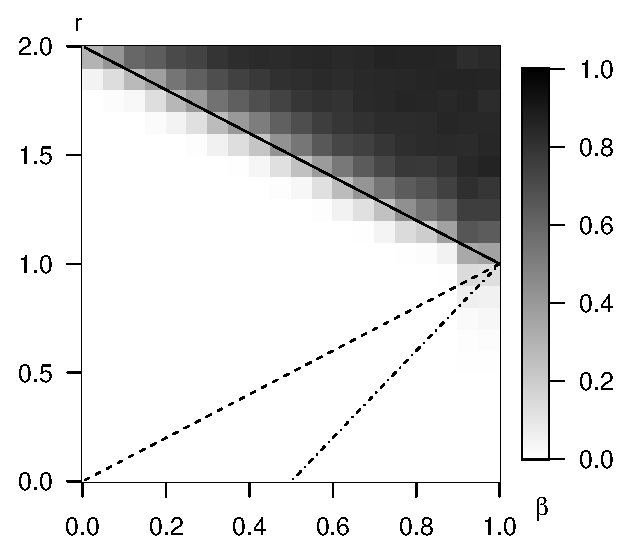
\includegraphics[width=0.4\textwidth]{./figures/simulated_boundaries/simulated_phase_diagram_Laplace_p10000_4.eps}
      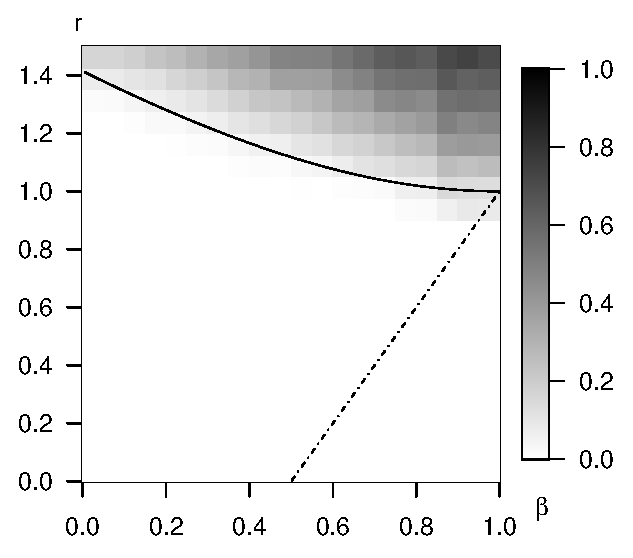
\includegraphics[width=0.4\textwidth]{./figures/simulated_boundaries/simulated_phase_diagram_NLC_p100.eps}
      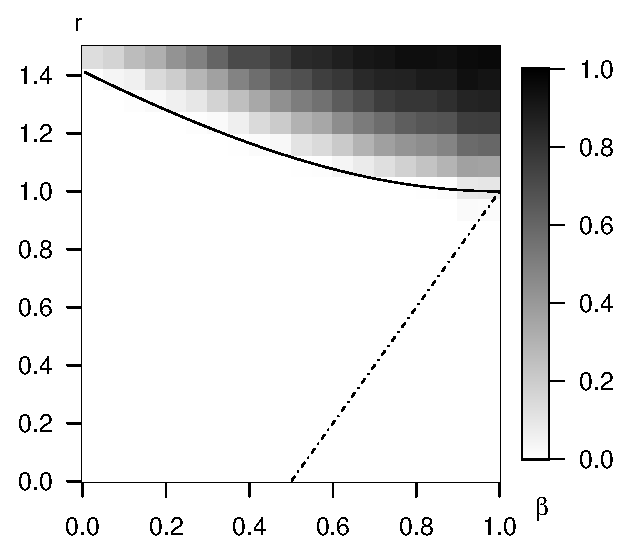
\includegraphics[width=0.4\textwidth]{./figures/simulated_boundaries/simulated_phase_diagram_NLC_p10000.eps}
      \caption{The empirical probability of exact support recovery from numerical experiments, as a function of sparsity level $\beta$ and signal sizes $r$, from Gaussian error models (upper panels), Laplace error models (middle panels), and generalized Gaussian with $\nu=1/2$ (lower panels); darker color indicates higher probability of exact support recovery. 
      The experiments were repeated 1000 times for each sparsity-signal size combination, and for dimensions $p=100$ (left panels) and $p=10000$ (right panels). Numerical results agree with the boundaries described in Theorem \ref{thm:sufficient}; convergence is noticeably slower for under generalized Gaussian ($\nu=1/2$) errors.
      For reference, the dashed and dash-dotted lines represent the weak classification and detection boundaries (see Chapter \ref{chap:phase-transitions}).}
      \label{fig:phase-simulated}
\end{figure}

